\chapter{Data and Methodology}
\label{chap:met}

\section{Raw Data}

The data originates from two sources. The first and most important source is Thomson Reuters Datastream. It covers publicly traded shares from developed countries of Europe, Japan and Asia-Pacific (Australia, New Zealand, Hong Kong, and Singapore) and contains the firms' yearly accounting figures and daily market information (e.g., price and volume).  The second data source is Institutional Brokers’ Estimate System (I/B/E/S) from Wharton Research Data Services, which provides analysts' forecasts. 

The firms are filtered based on [TODO add source of filtering methods].  
The final sample includes 8350 companies.


\section{Anomalies Data}
The anomaly dataset consists of 153 anomalies published in leading financial and accounting journals. The data is monthly and spans from January 1990 to December 2018. It covers the same 8350 firms as the raw data, totaling 1,607,117 observations. 

The anomalies can be classified into three groups: Fundamentals, Frictions, and I/B/E/S anomalies. Fundamental anomalies are primarily calculated from yearly accounting statements and are exemplified by Total Accruals, Asset Growth, or Leverage. Fundamental anomalies fall into 5 broad categories: Accruals (e.g., Total Accruals, Change in Common Equity, Inventory Growth), Investment (e.g., Asset Growth, Debt Issuance, Net Operating Assets), Intangibles (e.g., Asset Liquidity, Earnings Persistence, Herfindahl Index), Profitability (e.g., Profit Margin, Return-on-Equity, Capital Turnover) and Value (e.g., Enterprise Multiple, Assets-to-Market, or Net Payout Yield). Friction anomalies are primarily calculated from daily market data. For example, they include Bid-Ask Spread, 11-Month Residual Momentum, 52-Week-High, and Long-Term Reversal. I/B/E/S anomalies are calculated from the I/B/E/S dataset and cover analysts' forecasts and recommendations, such as Analyst Value, Change in Recommendation, or Forecast Dispersion. There are 93 Fundamentals, 48 Frictions and 12 I/B/E/S anomalies. Within the Fundamentals category, there are 21 Accruals, 15 Investment, 25 Intangibles, 18 Profitability, and 14 Value anomalies.  

A complete list of the anomalies can be found in the Appendix. [TODO]. 

Figures \ref{fig:corrplot_funds}, \ref{fig:corrplot_frictions}, and \ref{fig:corrplot_ibes} show plots of correlation matrices of Fundamental, Frictions, and I/B/E/S anomalies respectively. Correlations between variables from different categories are not shown, as they are all very low but for negligible exceptions. 


\begin{center}
	\begin{figure}
		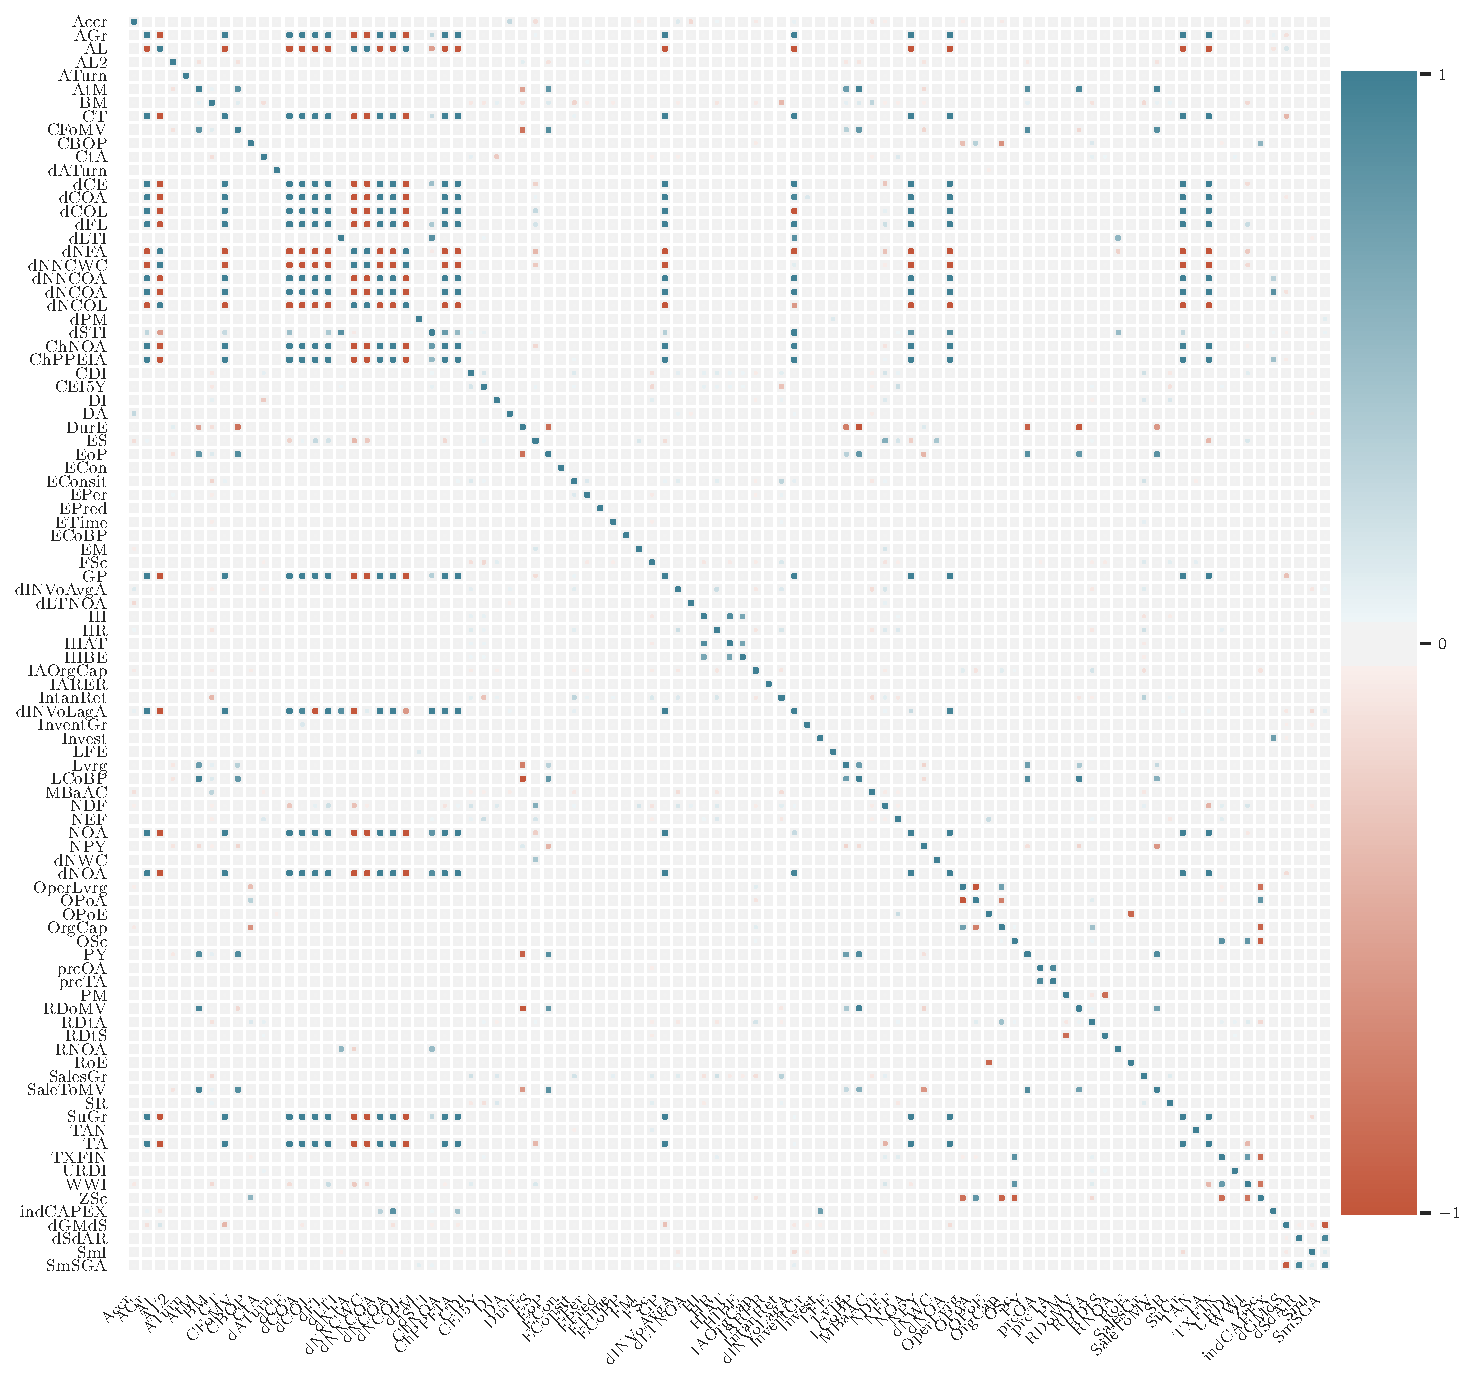
\includegraphics[width=\textwidth,height=\textheight,keepaspectratio]{Figures/corrplot_funds.pdf}
		\caption{Correlation Matrix of Fundamental Anomalies}
		\label{fig:corrplot_funds}
	\end{figure}
\end{center}

\begin{center}
	\begin{figure}
		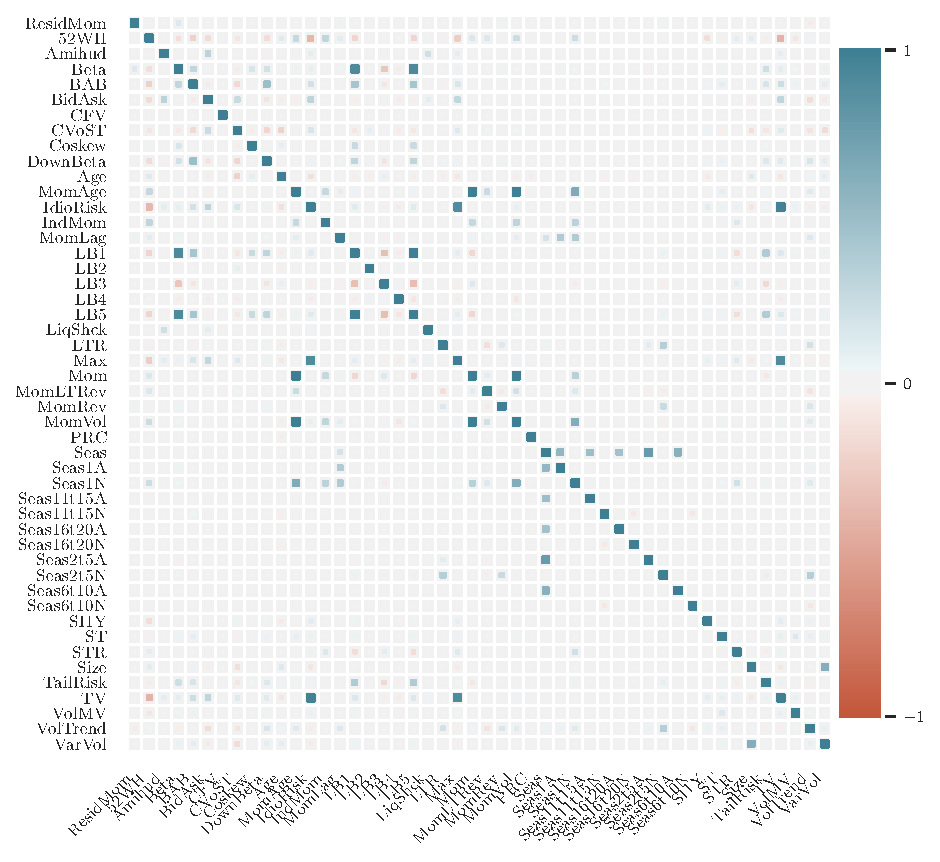
\includegraphics[width=\textwidth,height=\textheight,keepaspectratio]{Figures/corrplot_frictions.pdf}
		\caption{Correlation Matrix of Frictions Anomalies}
		\label{fig:corrplot_frictions}
	\end{figure}
\end{center}


\begin{center}
	\begin{figure}
		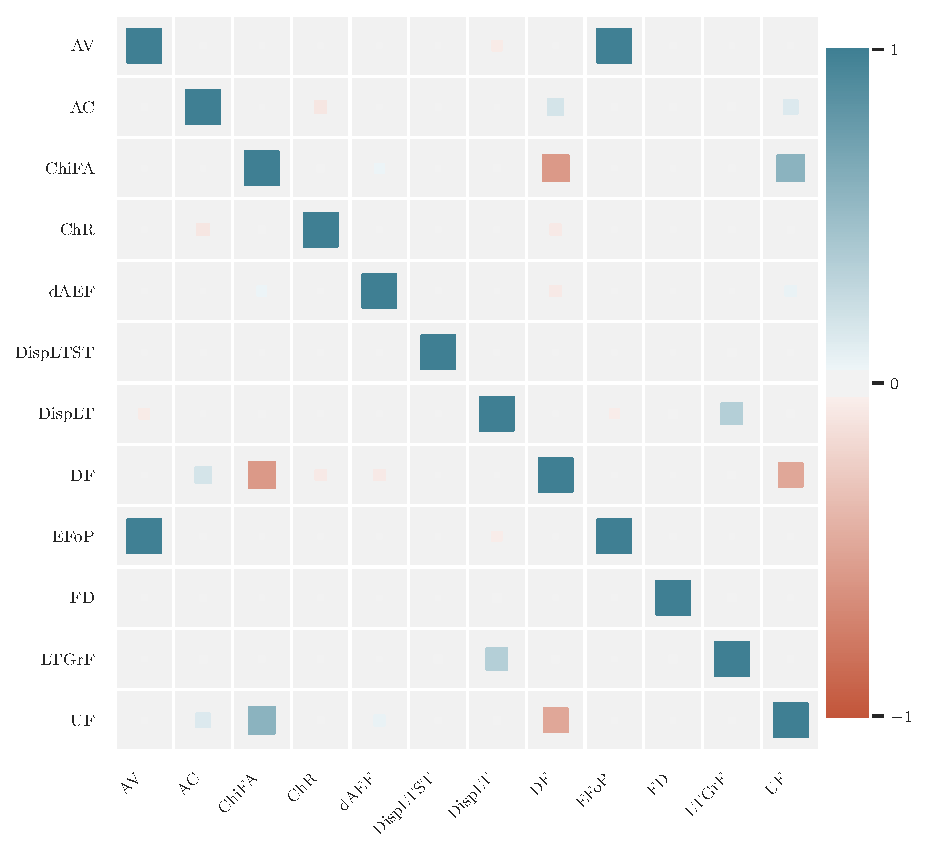
\includegraphics{Figures/corrplot_ibes.pdf}
		\caption{Correlation Matrix of I/B/E/S Anomalies}
		\label{fig:corrplot_ibes}
	\end{figure}
\end{center}
	

Figure \ref{fig:hist_returns} shows histogram of monthly returns 


\begin{center}
	\begin{figure}
		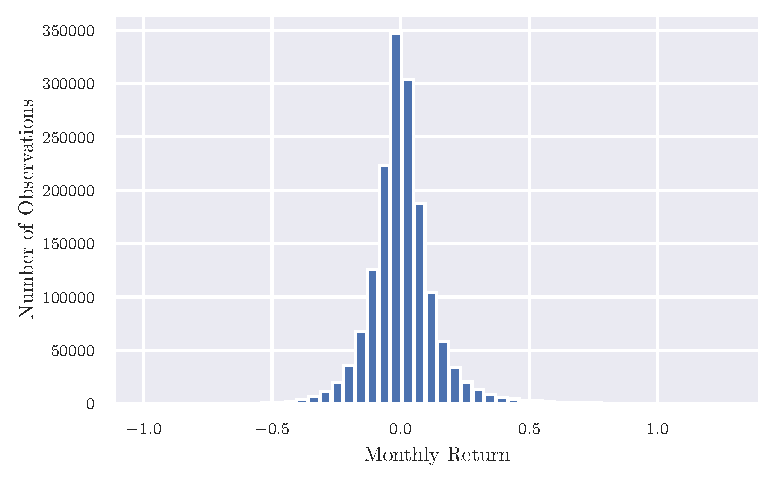
\includegraphics{Figures/hist_returns.pdf}
		\caption{Histogram of Monthly Returns}
		\label{fig:hist_returns}
	\end{figure}
\end{center}



